% !TEX TS-program = pdflatexmk
% ============================================================
%  Weetjes & Formules – Hoofdstuk 5: Hemelmechanica
%  C004206A – Sterren en Planeten  |  AJ 2025-26
% ============================================================
\documentclass[11pt, a4paper]{article}

% --- taal & codering ---
%\usepackage[english]{babel}
\usepackage[T1]{fontenc}
\usepackage[utf8]{inputenc}

% --- wiskunde ---
\usepackage{amsmath, amssymb, mathtools}

% --- opmaak ---
\usepackage[margin=2.2cm, top=2.5cm, bottom=2.5cm]{geometry}
\usepackage{booktabs, array, multirow, longtable}
\usepackage{xcolor}
\usepackage{enumitem}
%\usepackage{microtype}
\usepackage{parskip}
\usepackage{titlesec}
\usepackage{fancyhdr}
\usepackage{tikz}
\usetikzlibrary{arrows.meta, calc, decorations.markings}

% --- gekleurde kaders ---
\usepackage{tcolorbox}
\tcbuselibrary{skins, breakable, theorems}

% Kleurenpalet
\definecolor{blauw}{RGB}{0,70,140}
\definecolor{groen}{RGB}{0,110,60}
\definecolor{rood}{RGB}{180,30,30}
\definecolor{oranje}{RGB}{200,100,0}
\definecolor{paars}{RGB}{100,0,150}
\definecolor{lichtblauw}{RGB}{230,240,255}
\definecolor{lichtgroen}{RGB}{230,248,238}
\definecolor{lichtrood}{RGB}{255,235,235}
\definecolor{lichtoranje}{RGB}{255,245,225}
\definecolor{lichtpaars}{RGB}{245,235,255}
\definecolor{grijs}{RGB}{100,100,100}

% --- kader-stijlen ---
\newtcolorbox{formule}[1][]{
  enhanced, breakable,
  colback=lichtblauw, colframe=blauw,
  fonttitle=\bfseries\color{white},
  attach boxed title to top left={yshift=-2mm, xshift=4mm},
  boxed title style={colback=blauw, sharp corners},
  sharp corners=south, title={#1}
}
\newtcolorbox{weetje}[1][]{
  enhanced, breakable,
  colback=lichtgroen, colframe=groen,
  fonttitle=\bfseries\color{white},
  attach boxed title to top left={yshift=-2mm, xshift=4mm},
  boxed title style={colback=groen, sharp corners},
  sharp corners=south, title={#1}
}
\newtcolorbox{opgelet}[1][]{
  enhanced, breakable,
  colback=lichtrood, colframe=rood,
  fonttitle=\bfseries\color{white},
  attach boxed title to top left={yshift=-2mm, xshift=4mm},
  boxed title style={colback=rood, sharp corners},
  sharp corners=south, title={#1}
}
\newtcolorbox{tip}[1][]{
  enhanced, breakable,
  colback=lichtoranje, colframe=oranje,
  fonttitle=\bfseries\color{white},
  attach boxed title to top left={yshift=-2mm, xshift=4mm},
  boxed title style={colback=oranje, sharp corners},
  sharp corners=south, title={#1}
}
\newtcolorbox{afleiding}[1][]{
  enhanced, breakable,
  colback=lichtpaars, colframe=paars,
  fonttitle=\bfseries\color{white},
  attach boxed title to top left={yshift=-2mm, xshift=4mm},
  boxed title style={colback=paars, sharp corners},
  sharp corners=south, title={#1}
}

% --- sectietitels ---
\titleformat{\section}{\large\bfseries\color{blauw}}{}{0em}{}[\color{blauw}\titlerule]
\titleformat{\subsection}{\normalsize\bfseries\color{groen}}{}{0em}{}

% --- kop- en voettekst ---
\pagestyle{fancy}
\fancyhf{}
\lhead{\textcolor{grijs}{\small C004206A – Sterren en Planeten}}
\rhead{\textcolor{grijs}{\small H5: Hemelmechanica}}
\cfoot{\textcolor{grijs}{\small \thepage}}
\renewcommand{\headrulewidth}{0.4pt}

% --- handige macro's ---
\newcommand{\dd}{\mathrm{d}}
\newcommand{\AstrE}{\mathrm{AE}}
\newcommand{\zon}{\odot}
\newcommand{\aarde}{\oplus}
\newcommand{\maan}{\mathbb{C}}
\newcommand{\vecr}{\vec{r}}
\newcommand{\vecv}{\dot{\vec{r}}}
\newcommand{\veck}{\vec{k}}
\newcommand{\vece}{\vec{e}}
\newcommand{\dotprod}[2]{\vec{#1}\cdot\vec{#2}}

% ============================================================
\begin{document}
% ============================================================

\begin{center}
  {\LARGE\bfseries\color{blauw} Weetjes \& Formules}\\[4pt]
  {\large Hoofdstuk 5 – Hemelmechanica}\\[2pt]
  {\normalsize C004206A – Sterren en Planeten \quad|\quad AJ 2025--26}
\end{center}
\vspace{0.3cm}
\hrule height 2pt \vspace{0.5cm}

\tableofcontents
\newpage

% ============================================================
\section{Het gravitationeel tweelichamenprobleem}
% ============================================================

Twee massa's $m_1$ en $m_2$ in elkaars zwaartekrachtveld. De \textbf{relatieve plaatsvector}
$\vec{r} = \vec{r}_2 - \vec{r}_1$ (van $m_1$ naar $m_2$) voldoet aan:

\begin{formule}[Bewegingsvergelijking]
\[
  \ddot{\vec{r}} = -\frac{\mu}{r^3}\,\vec{r}
  \qquad \text{met} \quad \mu = G(m_1 + m_2)
\]
\end{formule}

\begin{weetje}[Wanneer $\mu \approx GM_1$?]
Als $m_2 \ll m_1$ (bv.\ satelliet om de aarde, planeet om de zon), dan
\[
  \mu = G(m_1 + m_2) \approx G m_1
\]
Dit is de benadering die je in bijna alle oefeningen mag gebruiken.
\end{weetje}

\begin{weetje}[Nuttige getalletjes]
\renewcommand{\arraystretch}{1.3}
\begin{tabular}{ll}
  $G = 6.674 \times 10^{-11}\ \mathrm{m^3\,kg^{-1}\,s^{-2}}$ & gravitatieconstante \\
  $\mu_\oplus = GM_\oplus = 3.986 \times 10^{14}\ \mathrm{m^3\,s^{-2}}$ & aarde \\
  $\mu_\odot = GM_\odot = 1.327 \times 10^{20}\ \mathrm{m^3\,s^{-2}}$ & zon \\
  $\mu_\mathbb{C} = GM_\mathbb{C} = 4.904 \times 10^{12}\ \mathrm{m^3\,s^{-2}}$ & maan \\
  $M_\oplus = 5.972 \times 10^{24}\ \mathrm{kg}$ & $R_\oplus = 6371\ \mathrm{km}$ \\
  $1\ \AstrE = 1.496 \times 10^{11}\ \mathrm{m}$ & $1\ \mathrm{parsec} = 206265\ \AstrE$ \\
\end{tabular}
\end{weetje}

% ============================================================
\section{Behouden grootheden}
% ============================================================

Het tweelichamenprobleem heeft \textbf{zes} onafhankelijke constanten van de beweging.

\subsection{Draaimoment $\vec{k}$}

\begin{formule}[Draaimoment per massa-eenheid]
\[
  \vec{k} = \vec{r} \times \dot{\vec{r}}
  \qquad \Rightarrow \qquad \dot{\vec{k}} = \vec{0}
\]
\end{formule}

\begin{weetje}[Gevolg: beweging in een vlak]
Omdat $\vec{k}$ constant is, liggen $\vec{r}$ en $\dot{\vec{r}}$ altijd in het vlak \emph{loodrecht} op $\vec{k}$.
\textbf{De baan ligt volledig in één vlak.}
\end{weetje}

De \textbf{grootte} van het draaimoment is:
\[
  k = r\,v_\perp = r^2\,\dot{f}
\]
waarbij $v_\perp$ de snelheidscomponent loodrecht op $\vec{r}$ is, en $\dot{f}$ de hoeksnelheid van de voerstraal.

\subsection{Energie $h$}

\begin{formule}[Specifieke mechanische energie (per massa-eenheid)]
\[
  \boxed{h = \frac{1}{2}v^2 - \frac{\mu}{r}}
\]
\begin{itemize}[leftmargin=1.5em, itemsep=1pt]
  \item $h < 0$: \textbf{gebonden baan} (ellips of cirkel)
  \item $h = 0$: \textbf{parabolische baan} (ontsnappingssnelheid exact bereikt)
  \item $h > 0$: \textbf{ongebonden baan} (hyperbool)
\end{itemize}
\end{formule}

\subsection{Laplace-Runge-Lenzvector $\vec{e}$}

\begin{formule}[LRL-vector]
\[
  -\mu\,\vec{e} = \vec{k} \times \dot{\vec{r}} + \mu\,\frac{\vec{r}}{r}
\]
\begin{itemize}[leftmargin=1.5em, itemsep=1pt]
  \item $\vec{e}$ ligt in het baanvlak, loodrecht op $\vec{k}$
  \item $|\vec{e}| = e$ = eccentriciteit van de baan
  \item $\vec{e}$ wijst van $m_1$ naar het \textbf{pericentrum}
\end{itemize}
\end{formule}

\begin{afleiding}[Relatie tussen $e$, $k$ en $h$]
\[
  \mu^2(e^2 - 1) = 2k^2 h
\]
Dit verband koppelt de drie behouden grootheden en toont dat slechts \textbf{vijf} ervan onafhankelijk zijn.
\end{afleiding}

% ============================================================
\section{Baanvergelijking en baantypes}
% ============================================================

\begin{formule}[Baanvergelijking (kegelsnede)]
\[
  \boxed{r = \frac{a(1-e^2)}{1 + e\cos f} = \frac{k^2/\mu}{1 + e\cos f}}
\]
$f$ = ware anomalie (gemeten vanuit $m_1$, nul bij pericentrum).
\end{formule}

\begin{center}
\renewcommand{\arraystretch}{1.5}
\begin{tabular}{cccc}
\toprule
\textbf{Eccentriciteit} & \textbf{Baantype} & \textbf{Energie} & \textbf{Gebonden?} \\
\midrule
$e = 0$ & Cirkel & $h = -\mu/(2a) < 0$ & Ja \\
$0 < e < 1$ & Ellips & $h = -\mu/(2a) < 0$ & Ja \\
$e = 1$ & Parabool & $h = 0$ & Nee (grens) \\
$e > 1$ & Hyperbool & $h = +\mu/(2a) > 0$ & Nee \\
\bottomrule
\end{tabular}
\end{center}

% ============================================================
\section{Ellipsbaan: sleutelformules}
% ============================================================

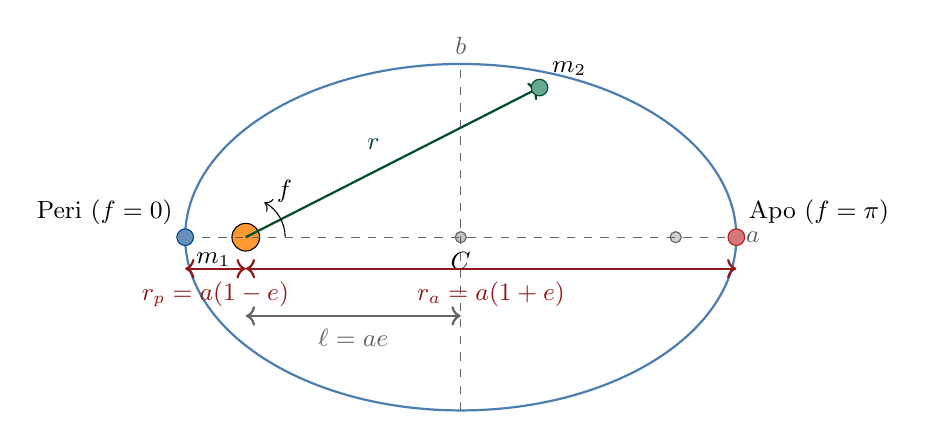
\begin{tikzpicture}[scale=1.0]
  % ellips
  \def\a{3.5} \def\b{2.2} \def\e{0.78}
  \def\c{2.73} % c = a*e
  % Teken ellips
  \draw[thick, color=blauw!70] (0,0) ellipse (\a cm and \b cm);
  % Brandpunt (zon/planeet)
  \filldraw[fill=orange!80, draw=black] (-\c,0) circle (5pt) node[below left=2pt]{\small $m_1$};
  % Centrum
  \filldraw[fill=grijs!40, draw=grijs] (0,0) circle (2pt) node[below=2pt]{\small $C$};
  % Lege brandpunt
  \filldraw[fill=grijs!30, draw=grijs] (\c,0) circle (2pt);
  % Assen
  \draw[dashed, grijs] (-\a,0) -- (\a,0) node[right]{\small $a$};
  \draw[dashed, grijs] (0,-\b) -- (0,\b) node[above]{\small $b$};
  % Pericentrum en apocentrum
  \filldraw[fill=blauw!60, draw=blauw] (-\a,0) circle (3pt) node[above left=1pt]{\small Peri ($f=0$)};
  \filldraw[fill=rood!60, draw=rood] (\a,0) circle (3pt) node[above right=1pt]{\small Apo ($f=\pi$)};
  % Voerstraal naar een punt
  \def\fx{1.0} \def\fy{1.9}
  \draw[thick, groen!70!black, ->] (-\c,0) -- (\fx,\fy) node[midway, above left=1pt]{\small $r$};
  \filldraw[fill=groen!60, draw=groen!70!black] (\fx,\fy) circle (3pt) node[above right=1pt]{\small $m_2$};
  % Hoek f
  \draw[->] (-\c+0.5,0) arc (0:62:0.5) node[right=1pt, yshift=4pt]{\small $f$};
  % Afstandslabels
  \draw[<->, thick, rood!80!black] (-\a,-0.4) -- (-\c,-0.4)
      node[midway, below=1pt]{\small $r_p = a(1-e)$};
  \draw[<->, thick, rood!80!black] (-\c,-0.4) -- (\a,-0.4)
      node[midway, below=1pt]{\small $r_a = a(1+e)$};
  % ℓ = ae label
  \draw[<->, thick, grijs] (0, -1.0) -- (-\c,-1.0) node[midway, below=1pt]{\small $\ell = ae$};
\end{tikzpicture}

\begin{formule}[Pericenter- en apocentrumsafstanden]
\[
  r_p = a(1-e) \qquad r_a = a(1+e)
\]
\[
  \boxed{a = \frac{r_p + r_a}{2}} \qquad \boxed{e = \frac{r_a - r_p}{r_a + r_p}}
\]
\end{formule}

\begin{formule}[Halve korte as en parametercombinaties]
\[
  b = a\sqrt{1-e^2}
  \qquad \ell = ae \quad\text{(afstand centrum–brandpunt)}
\]
\[
  k^2 = \mu\,a(1-e^2) \qquad h = -\frac{\mu}{2a}
\]
\end{formule}

\begin{weetje}[Twee manieren om $a$ en $e$ te vinden]
\textbf{Uit $r_p$ en $r_a$:}
\[ a = \tfrac{1}{2}(r_p + r_a), \qquad e = \tfrac{r_a - r_p}{r_a + r_p} \]
\textbf{Uit energie en draaimoment:}
\[ a = -\frac{\mu}{2h}, \qquad e = \sqrt{1 + \frac{2k^2 h}{\mu^2}} \]
\end{weetje}

% ============================================================
\section{Vis-viva-vergelijking en snelheden}
% ============================================================

\begin{formule}[Vis-viva-vergelijking (snelheid op elke positie)]
\[
  \boxed{v^2 = \mu\left(\frac{2}{r} - \frac{1}{a}\right)}
\]
Geldig voor ellips ($a>0$) én hyperbool ($a>0$, maar schrijf $h=+\mu/(2a)$).
\end{formule}

\begin{afleiding}[Afleiding]
Uit energiebehoud: $\tfrac{1}{2}v^2 - \mu/r = h = -\mu/(2a)$, dus
$v^2 = 2\mu/r - \mu/a$.
\end{afleiding}

\begin{formule}[Snelheden bij pericentrum en apocentrum]
Bij peri- en apocentrum staat $\vec{v}$ loodrecht op $\vec{r}$, dus $v = k/r$:
\begin{align}
  v_p &= \sqrt{\frac{\mu}{a}\cdot\frac{1+e}{1-e}} = \sqrt{\frac{\mu(1+e)}{a(1-e)}} \\[6pt]
  v_a &= \sqrt{\frac{\mu}{a}\cdot\frac{1-e}{1+e}} = \sqrt{\frac{\mu(1-e)}{a(1+e)}}
\end{align}
\end{formule}

\begin{formule}[Cirkelbaan ($e = 0$, $r = a = $ const)]
\[
  v_\mathrm{circ} = \sqrt{\frac{\mu}{r}}
  \qquad
  T_\mathrm{circ} = \frac{2\pi r}{v_\mathrm{circ}} = 2\pi\sqrt{\frac{r^3}{\mu}}
\]
\end{formule}

\begin{formule}[Ontsnappingssnelheid (parabolische grens, $h=0$)]
\[
  v_\mathrm{esc} = \sqrt{\frac{2\mu}{r}} = \sqrt{2}\;v_\mathrm{circ}
\]
\end{formule}

\begin{weetje}[Snelheidscomponenten op een ellipsbaan]
Splits de snelheid in een \textbf{radiële} component $v_r = \dot{r}$ en een \textbf{tangentiële} component $v_f = r\dot{f}$:
\[
  v_r = \frac{\mu}{k}\,e\sin f
  \qquad
  v_f = \frac{\mu}{k}(1 + e\cos f)
  \qquad
  v^2 = v_r^2 + v_f^2
\]
Bij pericenter: $v_r = 0$, $v_f = v_p$. \quad Bij apocenter: $v_r = 0$, $v_f = v_a$.\\
\textbf{Impuls langs de baan:} $\Delta v = v_\mathrm{nieuw} - v_\mathrm{oud}$ verandert $a$ en $e$.
\end{weetje}

\begin{tip}[Deltasnelheid bij een manoeuvre]
Bij een \textbf{raketverbranding} (instantaan, richting onveranderd) verandert enkel de grootte van $\vec{v}$ op het moment van verbranding. Nieuwe $a$ en $e$ berekenen via:
\[
  h_\mathrm{nieuw} = \tfrac{1}{2}v_\mathrm{nieuw}^2 - \mu/r
  \qquad \Rightarrow \qquad a_\mathrm{nieuw} = -\mu/(2h_\mathrm{nieuw})
\]
Dan $e_\mathrm{nieuw}$ via de pericenter/apocentrumafstanden (als de verbranding aan peri of apo plaatsvindt, blijft die afstand vast).
\end{tip}

% ============================================================
\section{Wetten van Kepler}
% ============================================================

\begin{formule}[Eerste wet van Kepler]
\textit{De baan van een planeet is een ellips met de zon in één van de brandpunten.}\\[4pt]
(Meer algemeen: de baan is een kegelsnede met $m_1$ in het brandpunt.)
\end{formule}

\begin{formule}[Tweede wet van Kepler (behoud van draaimoment)]
\textit{De voerstraal bestrijkt gelijke oppervlakken in gelijke tijdsintervallen.}
\[
  \frac{\dd A}{\dd t} = \frac{k}{2} = \mathrm{const}
\]
Gevolg: het object beweegt \textbf{sneller bij pericentrum} en trager bij apocentrum.
\end{formule}

\begin{formule}[Derde wet van Kepler]
\[
  \boxed{P^2 = \frac{4\pi^2}{\mu}\,a^3}
\]
\begin{itemize}[leftmargin=1.5em, itemsep=2pt]
  \item Geldt voor elke ellipsbaan, ongeacht $e$.
  \item Voor het zonnestelsel ($m_2 \ll M_\odot$): $P^2 \propto a^3$ (universeel voor alle planeten).
  \item Massa van het centrale lichaam: $M = \frac{4\pi^2\,a^3}{G\,P^2}$.
\end{itemize}
\end{formule}

\begin{weetje}[Gemiddelde hoeksnelheid]
\[
  n = \frac{2\pi}{P} = \sqrt{\frac{\mu}{a^3}} \quad [\mathrm{rad/s}]
\]
Dit is de \emph{middelbare} hoeksnelheid. De werkelijke hoeksnelheid $\dot{f}$ varieert langs de baan.
\end{weetje}

% ============================================================
\section{Tijdsrekening op de ellipsbaan}
% ============================================================

\subsection{De drie anomalieën}

\begin{formule}[Middelbare anomalie $M$ (neemt lineair toe)]
\[
  M = n(t - \tau) = \frac{2\pi}{P}(t - \tau)
\]
$\tau$ = tijdstip van pericentrumdoorgang. $M = 0$ bij pericentrum, $M = 2\pi$ na één periode.
\end{formule}

\begin{formule}[Eccentrische anomalie $E$ (meetbaar vanuit centrum ellips)]
Positie van $m_2$ in cartesische coördinaten (oorsprong = brandpunt $m_1$):
\begin{align}
  x &= a(\cos E - e) \\
  y &= a\sqrt{1-e^2}\,\sin E = b\sin E \\
  r &= a(1 - e\cos E)
\end{align}
\end{formule}

\begin{formule}[Vergelijking van Kepler (verbindt $E$ en $M$)]
\[
  \boxed{E - e\sin E = M(t) = \frac{2\pi}{P}(t - \tau)}
\]
Dit is \textbf{transcendentaal}: geen gesloten oplossing voor $E$ als functie van $M$.
\end{formule}

\begin{formule}[Ware anomalie $f$ uit $E$ (of omgekeerd)]
\[
  \tan\frac{f}{2} = \sqrt{\frac{1+e}{1-e}}\;\tan\frac{E}{2}
\]
\end{formule}

\subsection{Kepler-vergelijking oplossen (iteratief)}

\begin{tip}[Methode 1: Eenvoudige iteratie]
Herschrijf als $E = M + e\sin E$ en itereer:
\[
  E_0 = M, \qquad E_{i+1} = M + e\sin E_i
\]
Convergeert voor kleine $e$. Stop als $|E_{i+1} - E_i| < $ gewenste nauwkeurigheid.
\end{tip}

\begin{tip}[Methode 2: Newton-Raphson (sneller)]
Definieer $f(E) = E - e\sin E - M = 0$, dan:
\[
  E_{i+1} = E_i - \frac{E_i - e\sin E_i - M}{1 - e\cos E_i}
  = E_i + \frac{M + e\sin E_i - E_i}{1 - e\cos E_i}
\]
Convergeert veel sneller, ook voor grote $e$.
\end{tip}

\begin{weetje}[Wat geeft de vergelijking van Kepler?]
\textbf{Gegeven:} baanelementen ($a$, $e$, $\tau$, $P$) + tijdstip $t$ \\
\textbf{Bereken:} $M \to E \to (x, y, r, f)$ = positie op de baan \\
De tijdsduur tussen twee anomaliewaarden $f_1$ en $f_2$ vind je via:
$\Delta t = \frac{P}{2\pi}(E_2 - e\sin E_2 - E_1 + e\sin E_1)$
\end{weetje}

% ============================================================
\section{De zes baanelementen}
% ============================================================

\begin{center}
\renewcommand{\arraystretch}{1.5}
\begin{tabular}{cp{5cm}p{7cm}}
\toprule
\textbf{Element} & \textbf{Naam} & \textbf{Beschrijving} \\
\midrule
$e$ & Eccentriciteit & Vorm van de baan: $e=0$ (cirkel), $0<e<1$ (ellips) \\
$a$ & Halve lange as & Grootte van de baan; bepaalt $P$ en $h$ \\
$i$ & Inclinatie & Kanteling baanvlak t.o.v.\ referentievlak ($0°=$ prograde; $90°=$ polair; $180°=$ retrograde) \\
$\Omega$ & Lengte klimmende knoop & Positie baanvlak in referentievlak (richting van klimmende knoop t.o.v.\ lentepunt) \\
$\omega$ & Argument pericentrum & Richting pericentrum in het baanvlak (hoek van klimmende knoop tot pericentrum) \\
$\tau$ & Tijdstip pericentrum & Tijdsas: wanneer is $m_2$ bij pericentrum? \\
\bottomrule
\end{tabular}
\end{center}

\begin{weetje}[Geheugensteuntje: vorm, grootte, oriëntatie, timing]
\begin{itemize}[leftmargin=1.5em, itemsep=2pt]
  \item \textbf{Vorm:} $e$ (hoe plat is de ellips?)
  \item \textbf{Grootte:} $a$ (hoe groot is de ellips?)
  \item \textbf{Ruimtelijke oriëntatie:} $i$ en $\Omega$ (hoe ligt het baanvlak?)
  \item \textbf{Positie in het vlak:} $\omega$ (hoe ligt de ellips in het vlak?)
  \item \textbf{Tijdsas:} $\tau$ (wanneer is het pericentrum?)
\end{itemize}
\end{weetje}

\begin{weetje}[Prograde vs.\ retrograde]
\begin{itemize}[leftmargin=1.5em, itemsep=1pt]
  \item $i \in [0°, 90°)$: \textbf{prograde} beweging (zelfde richting als referentie)
  \item $i = 90°$: \textbf{polaire baan} (loopt over de polen)
  \item $i \in (90°, 180°]$: \textbf{retrograde} beweging (omgekeerde richting)
\end{itemize}
In het zonnestelsel is het referentievlak het \textbf{eclipticavlak}; de referentiepool is de noordelijke ecliptische pool.
\end{weetje}

% ============================================================
\section{Speciale snelheidsrelaties}
% ============================================================

\begin{formule}[Snelheid bij perigeum uit energie en positie]
\[
  \frac{1}{2}v_p^2 = \frac{\mu}{r_p} - \frac{\mu}{2a}
  = \frac{\mu}{a}\cdot\frac{1+e}{2(1-e)}
  = \frac{\mu}{a(1-e)}\cdot\frac{1+e}{2} \cdot \frac{2}{1}
\]
Compact:
\[
  v_p = \sqrt{\frac{\mu}{a}\cdot\frac{1+e}{1-e}}
\]
\end{formule}

\begin{formule}[Behoud van draaimoment: snelheidsproduct]
\[
  r_p\,v_p = r_a\,v_a = k
\]
Dit is handig om $v_a$ te berekenen als je $v_p$ al weet (of omgekeerd).
\end{formule}

\begin{formule}[Radiale snelheid op een willekeurige positie]
\[
  v_r = \frac{\mu}{k}\,e\sin f, \qquad v_\perp = \frac{\mu}{k}(1+e\cos f)
\]
\[
  v^2 = v_r^2 + v_\perp^2 = \frac{\mu^2}{k^2}\bigl(1 + 2e\cos f + e^2\bigr)
\]
Of gebruik gewoon vis-viva: $v^2 = \mu(2/r - 1/a)$.
\end{formule}

% ============================================================
\section{Siderische en synodische periode van planeten}
% ============================================================

\begin{formule}[Siderische vs.\ synodische periode]
\[
  \frac{1}{P_{12}} = \frac{1}{P_1} - \frac{1}{P_2}
  \qquad (P_1 < P_2, \text{ beide prograde})
\]
$P_{12}$ = synodische periode (tijd tussen twee opeenvolgende opposities/conjuncties).\\
$P_1$, $P_2$ = siderische periodes van de twee planeten.
\end{formule}

\begin{weetje}[Opposities en conjuncties]
\begin{itemize}[leftmargin=1.5em, itemsep=1pt]
  \item \textbf{Oppositie} (buitenplaneet): aarde tussen zon en planeet; ecliptische lengtes $180°$ uit elkaar.
  \item \textbf{Conjunctie} (buitenplaneet): zon tussen aarde en planeet; ecliptische lengtes gelijk.
  \item \textbf{Benedenconjunctie} (binnenplaneet): planeet voor de zon.
  \item \textbf{Bovenconjunctie} (binnenplaneet): planeet achter de zon.
  \item Retrograde beweging: rondom oppositie (buitenplaneet) of benedenconjunctie (binnenplaneet).
\end{itemize}
\end{weetje}

% ============================================================
\section{Hyperboolbaan}
% ============================================================

\begin{formule}[Hyperbool ($e > 1$, $h > 0$)]
\[
  r = \frac{a(e^2-1)}{1+e\cos f}
  \qquad
  h = +\frac{\mu}{2a} > 0
  \qquad
  r_p = a(e-1)
\]
$f$ loopt van $-f_\infty$ tot $+f_\infty$ met $\cos f_\infty = -1/e$ (asymptoten).
\end{formule}

\begin{formule}[Snelheid op oneindig (hyperbolische overmaatsnelheid)]
\[
  v_\infty = \sqrt{2h} = \sqrt{\frac{\mu}{a}}
\]
Dit is de snelheid ver van het centrale lichaam, \emph{voor} of \emph{na} het gravitationele slingeren.
\end{formule}

\begin{weetje}[``Komt van oneindig'']
In de Artemis-oefening en soortgelijke aanpakken: als een ruimteschip ``vanuit de verte'' een planeet benadert, dan is $v_\infty$ de snelheid van het schip t.o.v.\ de planeet op grote afstand. Bij pericentrum:
\[
  v_p = \sqrt{v_\infty^2 + v_\mathrm{esc}^2}
  = \sqrt{v_\infty^2 + \frac{2\mu}{r_p}}
\]
(volgt gewoon uit energiebehoud met $h = v_\infty^2/2$).
\end{weetje}

% ============================================================
\section{Snelle-referentietabel}
% ============================================================

\begin{center}
\renewcommand{\arraystretch}{1.6}
\begin{tabular}{p{5.5cm} p{8cm}}
\toprule
\textbf{Grootte} & \textbf{Formule} \\
\midrule
Halve lange as & $a = \tfrac{1}{2}(r_p + r_a)$ \\
Eccentriciteit & $e = (r_a - r_p)/(r_a + r_p)$ \\
Pericentrum & $r_p = a(1-e)$ \\
Apocentrum  & $r_a = a(1+e)$ \\
Halve korte as & $b = a\sqrt{1-e^2}$ \\
Energie & $h = -\mu/(2a)$ \quad (ellips) \\
Draaimoment² & $k^2 = \mu a(1-e^2)$ \\
Periode & $P = 2\pi\sqrt{a^3/\mu}$ \\
Massa centraal lichaam & $M = 4\pi^2 a^3/(GP^2)$ \\
Snelheid (vis-viva) & $v^2 = \mu(2/r - 1/a)$ \\
Snelheid cirkel & $v_c = \sqrt{\mu/r}$ \\
Ontsnappingssnelheid & $v_\mathrm{esc} = \sqrt{2\mu/r} = \sqrt{2}\,v_c$ \\
Snelheid bij pericentrum & $v_p = \sqrt{\mu(1+e)/[a(1-e)]}$ \\
Snelheid bij apocentrum & $v_a = \sqrt{\mu(1-e)/[a(1+e)]}$ \\
Draaimomentsrelatie & $r_p v_p = r_a v_a = k$ \\
Middelbare hoeksnelheid & $n = 2\pi/P = \sqrt{\mu/a^3}$ \\
Middelbare anomalie & $M = n(t-\tau)$ \\
Vergelijking van Kepler & $E - e\sin E = M$ \\
Positie op baan (excentrisch) & $r = a(1 - e\cos E)$ \\
Ware uit eccentrische anomalie & $\tan(f/2) = \sqrt{(1+e)/(1-e)}\tan(E/2)$ \\
Hyperbolische overmaatsnelheid & $v_\infty = \sqrt{\mu/a}$ \\
\bottomrule
\end{tabular}
\end{center}

% ============================================================
\section{Stappenplan voor typische oefeningen}
% ============================================================

\begin{tip}[Satelliet- of planeetbaan bepalen uit $r_p$ en $r_a$]
\begin{enumerate}[leftmargin=1.5em, itemsep=3pt]
  \item Bereken $a = \tfrac{1}{2}(r_p + r_a)$ en $e = (r_a - r_p)/(r_a + r_p)$.
  \item Bereken $P$ via derde wet: $P = 2\pi\sqrt{a^3/\mu}$.
  \item Bereken snelheden via vis-viva: $v^2 = \mu(2/r - 1/a)$.
\end{enumerate}
\end{tip}

\begin{tip}[Massa centraal lichaam bepalen]
\begin{enumerate}[leftmargin=1.5em, itemsep=3pt]
  \item Bepaal $a$ (uit $r_p$, $r_a$ of hoekgrootte + afstand).
  \item Meet $P$ (baanperiode van satelliet/maan).
  \item Bereken $M = 4\pi^2 a^3 / (G P^2)$.
\end{enumerate}
\end{tip}

\begin{tip}[Positie op baan op tijdstip $t$]
\begin{enumerate}[leftmargin=1.5em, itemsep=3pt]
  \item Bereken middelbare anomalie: $M = \tfrac{2\pi}{P}(t - \tau)$.
  \item Los Kepler-vergelijking op: $E - e\sin E = M$ (iteratief).
  \item Bereken $r = a(1-e\cos E)$ en $f$ via $\tan(f/2) = \sqrt{(1+e)/(1-e)}\tan(E/2)$.
  \item Cartesisch: $x = a(\cos E - e)$, $y = b\sin E$.
\end{enumerate}
\end{tip}

\begin{tip}[Tijdsduur tussen twee baanposities]
\begin{enumerate}[leftmargin=1.5em, itemsep=3pt]
  \item Zet de twee ware anomalieën $f_1$, $f_2$ om naar eccentrische anomalieën $E_1$, $E_2$.
  \item Bereken $M_1 = E_1 - e\sin E_1$ en $M_2 = E_2 - e\sin E_2$.
  \item Tijdsduur: $\Delta t = \tfrac{P}{2\pi}(M_2 - M_1)$ \quad (modulo volledige omwentelingen).
\end{enumerate}
\end{tip}

\begin{opgelet}[Veelgemaakte fouten]
\begin{itemize}[leftmargin=1.5em, itemsep=3pt]
  \item \textbf{Eenheden}: $\mu$ in $\mathrm{m^3/s^2}$, $r$ in $\mathrm{m}$, $P$ in seconden $\to$ dan $v$ in $\mathrm{m/s}$.
  \item \textbf{Hyperbool vs.\ ellips}: voor een hyperbool is $a > 0$ per definitie, maar $h = +\mu/(2a) > 0$.
  \item \textbf{Richting $\Delta v$}: een impuls die $v$ vergroot \emph{op de positie van de verbranding} verandert $a$ en $e$ maar \textbf{niet} de afstand op het moment van verbranding. Die positie blijft op de nieuwe baan liggen.
  \item \textbf{$m_1 \ll m_2$ of niet}: gebruik altijd $\mu = G(m_1 + m_2)$, tenzij de benadering expliciet gevraagd is.
  \item \textbf{Kepler in radialen}: $M$, $E$, $f$ altijd in radialen berekenen.
\end{itemize}
\end{opgelet}

\end{document}
